\documentclass[11pt, letterpaper, titlepage]{article}
\usepackage[utf8]{inputenc}
\usepackage[export]{adjustbox}
\usepackage{geometry}
 \geometry{
 a4paper,
 total={168mm,257mm},
 left=20mm,
 top=15mm,
 includefoot,includehead
 }
\usepackage[backend=biber, style=authoryear, giveninits=true, maxbibnames=25, uniquename=init, maxcitenames=2, hyperref=true, dashed=false]{biblatex}			% Benutze Biber/BibLaTeX zum Zitieren
\addbibresource{report_short.bib}
\renewcommand{\cite}{\parencite}
\usepackage{caption}
\usepackage{subcaption}
\usepackage{graphicx}
\usepackage{svg}
\usepackage{placeins}
\usepackage[hidelinks]{hyperref}
\usepackage{amsmath}
\usepackage[headsepline]{scrlayer-scrpage}
\usepackage{acronym}

\clearpairofpagestyles %Seitenzahl nicht in der Kopfzeile

\title{MeetEU Project - Team Heidelberg - Team 1 -- \\ Identification and Enhancement of novel Sars-CoV-2 NSP13 Helicase Inhibitors}
\author{Linda Blaier, Paul Brunner, Selina Ernst, Valerie Segatz, and Chlo\'{e} Weiler}
\date{February 2024}

\begin{document}

\maketitle

\ihead{\headmark}
\automark{section}  %Kopfzeile gleich dem Sektiontitel
\cfoot{\pagemark}   %\ofood Seitenzahl rechts

\section{Workflow}

\begin{figure}[h]
  \centering
  %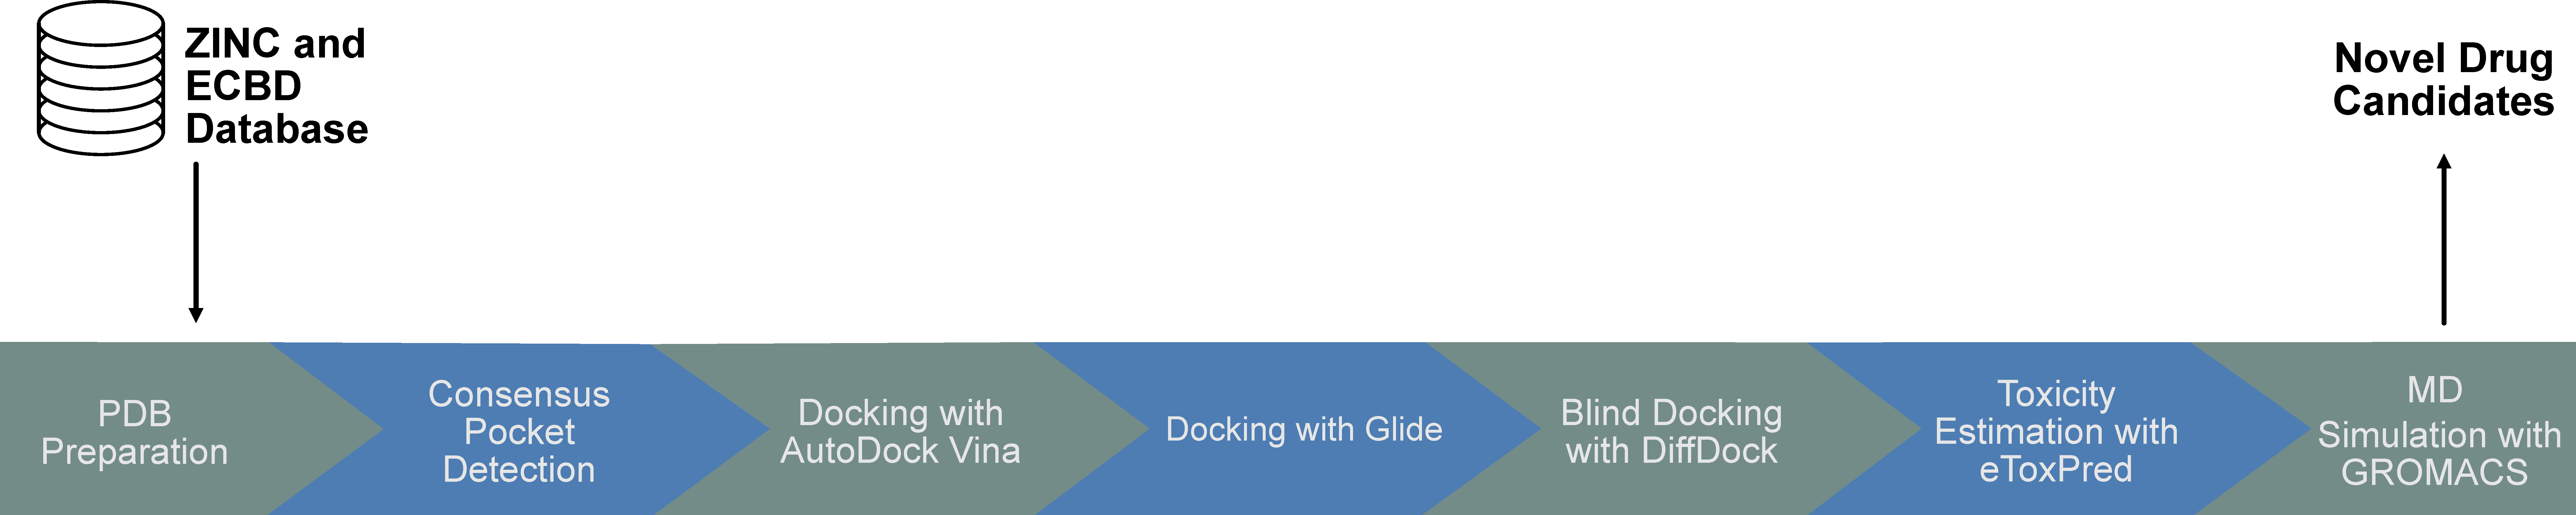
\includegraphics[width=\textwidth]{Workflow_MeetEU.pdf}
  \caption*{\textbf{Workflow for the discovery of NSP13 helicase inhibitors.}}
  \label{workflow}
\end{figure}

\setcounter{figure}{0}
\renewcommand{\thefigure}{\arabic{figure}}


\section{Material and Methods}
%\subsection{Datasets from ZINC20 and ECBD}
1616 FDA-approved drugs from the ZINC database \cite{Irwin.2020} and 5016 files from the ECBD pilot library were downloaded.
%\subsection{Receptor and Ligand Preparation}
Three protein structures of NSP13 (PDB codes: 6ZSL, 5RME, and 5RM2) were aquired from RCSB PDB. \\
\noindent For identification of the consensus pocket, the protein structures were prepared using \textit{PDBFixer} \cite{Eastman_2017}. \textit{Fpocket} \cite{package_Fpocket}, \textit{PrankWeb 3} \cite{package_P2Rank,package_PrankWeb,package_PrankWeb3}, and \textit{FTMap} \cite{package_FTMAP} were run on the structures to determine the consensus binding pocket. For further experiments, the docking box was set to be a cube with an edge length of 30 \AA. Molecular docking was performed on the A chain of 6ZSL whose catalytic activity had been confirmed in previous publications \cite{Berta_2021}. Molecular docking of the ligands was performed using \textit{AutoDock Vina} \cite{Trott.2010} and \textit{Glide} \cite{Friesner2004}. The docking results were then validated through blind docking with \textit{DiffDock} \cite{Corso.2022}. The toxicity and synthetic accessibility of the Top 100 scorers from \textit{AutoDock Vina} were predicted using \textit{eToxPred} \cite{pu2019toxpred}.
%\subsection{Molecular Dynamics Simulation}
In order to validate the binding of the top scorer, a molecular dynamics simulation was performed using \textit{Gromacs} \cite{packageGROMACS}.\\

\section{Results}
The location of our consensus pocket was found within the ATP binding site, between the RecA-like domains A1 and A2. The molecular docking with \textit{AutoDock Vina} indentified 100 top scorers, which were ranked by their binding affinity, ranging from -10.3 to -8.8 $\frac{kcal}{mol}$. Passing these top 100 compounds through \textit{Glide} returned the following top three compounds: ZINC000096077632 (popular name: Angiotensin 1-7), ZINC000008101127 and ZINC000035880991. While they exhibit good binding affinities, they still do not bind as well as ATP. \textit{DiffDock} did not predict our Top 1 Glide scorer within our binding box, however the molecular dynamics simulation suggested a stable bond between the ligand and the helicase in our consensus pocket, as the ligand stayed inside of the pocket through the whole simulation. Multiple hydrogen bonds can be observed at the end of the 100 ns simulation, which had almost all been previously found by \textit{Glide}. The estimation of toxicity and synthetic accessibility using \textit{eToxPred} showed that only one out of out top 100 compounds is predicted to be toxic. Furthermore, most of the compounds seem to be accessible in their synthesis.

\FloatBarrier

\section{Discussion and Outlook}
Molecular Docking was performed using the FDA approved ligands from ZINC and the pilot library from ECBD. The Top 100 Vina results were further analysed by Glide and their toxicity and synthetic accessibility estimated via eToxPred. Validation of our Top 10 scorer was achieved by blind docking with Diffdock and MD-Simulation using GROMACS. In conclusion, our findings suggest Angiotensin 1-7 as lead compound. This result is further supported by \textcite{angio}, who proposed Angiotensin 1-7 as a new therapy to support the recovery from Covid-19. Moreover, because of its role in the Renin-Angiotensin-Aldosteron System, it seemingly could also lower the viral damage to the body by inhibiting NSP13.\\

In comparison, Sorbonne team 5 used a pre selection of the ECBD pilot library and subjected these to Vina. For their first ranked ligand our results predict an affinity score of -11.1 and was ranked 63 in our Vina results. The remaining 7 were mapped to lower with ranks between 123 and 2626. These results however aren't surprising, as Sorbonne 5 used a different binding pocket, compared to us.\\

\subsection{Limitations of the project}
Regarding molecular dynamics (MD) simulation, the project was held back by the tight time schedule. Further simulations should have been performed in order to validate our pipeline and compare our top scorer. Moreover, since MD simulations are a very stochastic process, they should always be estimated using replicas. Multiple runs of the same simulation, using replica exchange with dynamical scaling \cite{REDS} could have therefore deepened our confidence in the results.\\
\\
Of further interest could have been the implementation of \textit{AutoGrow4} \cite{packageAutogrow4}. This could have helped, alongside toxicity and synthetic accessibility predictions via\textit{eToxPred} to improve our lead drugs and to generate novel compounds.

\pagebreak
\FloatBarrier
\renewcommand{\bibname}{References}  % damit Literatuverzeicnis mit "References" betitelt
\printbibliography



\end{document}
